\chapter{System and Context Boundaries}

\section{Stakeholder}
\begin{enumerate}
	\item kAlarm users
	\par Users who previously used kAlarm on linux, and wishing to find a similar but remastered and cross-platform software.
	\item Computer users
	\par Those who tend to forget many things.
	\item Investors
	\par Investors in the project. For example advertisers looking for visibility in the software.
	\item The GNU Project
	\par The GNU Project collective could be pleased to see that an updated version of kAlarm is proposed.
\end{enumerate}

\section{Actors}
\begin{enumerate}
	\item Software User (Primary Actor)
	\par The peoples who will  use the software. They are the first concerned  by the product.
	\item Administrator (Primary Actor)
	\par Super users with special authorizations. May be able to manipulate the data and the other users.
	\\ \textbf{It is likely that the software does not need an administrator.}
	\item System Time (Supporting Actor)
	\par The service specific to the OS and providing the exact international time.
	\item Messaging Software (Supporting Actor)
	\par Allows ClockAlarm to send Emails.
	\item OS Notification Services (Supporting Actor)
	\par OS specific notification center or notification service.
    \item OS File System (Supporting Actor)
    \par Allows ClockAlarm to load configuration and alert files.
\end{enumerate}


\newpage
\section{System context}
\begin{figure}[h]
	\centering
	\caption{System context}
	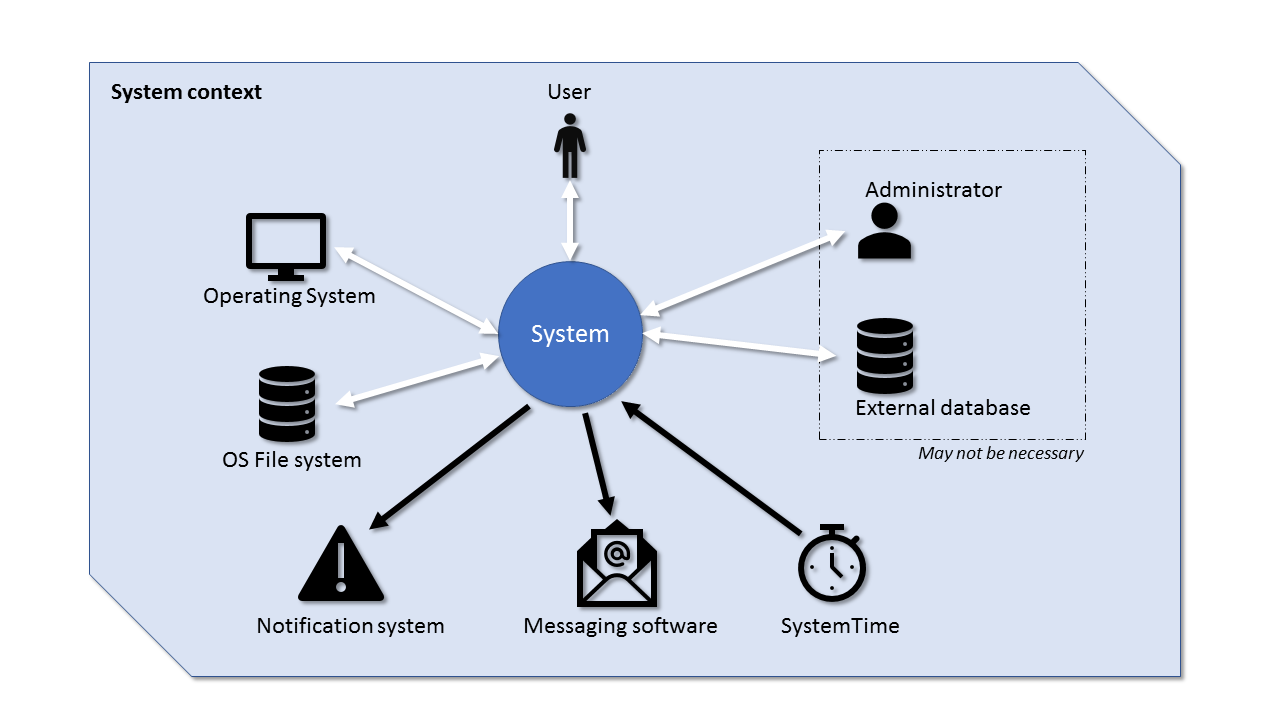
\includegraphics[width=0.7\textwidth]{systemcontext_diagram.png}
\end{figure}

\section{System boundary}
In addition to the elements above, special attention should be given to the following points.
\begin{itemize}
	\item The must-have goal isn't to add functionality to the existing software kAlarm, but to create a similar and cross-platform product.
	\item The existence of a database and an administrator could be dropped and go out of context.
	\item The software isn't meant to be an alternative to an agenda. It behaves like a list of tasks and reminders.
\end{itemize}

\section{Context boundary}
In addition to the logical considerations and those stated above, the following points should be taken into account.
\begin{itemize}
	\item The software is responsible for asking the messaging software to send to emails. This means that the way emails are sent isn't part of the environment.
	\item The software bases its alarms on the internal time. The accuracy of the time and of the time zone with respect to the geographical position of the machine is not part of the environment.
\end{itemize}